\begin{figure}[H]
		\begin{minipage}[t]{0.45\linewidth}
		\centering
		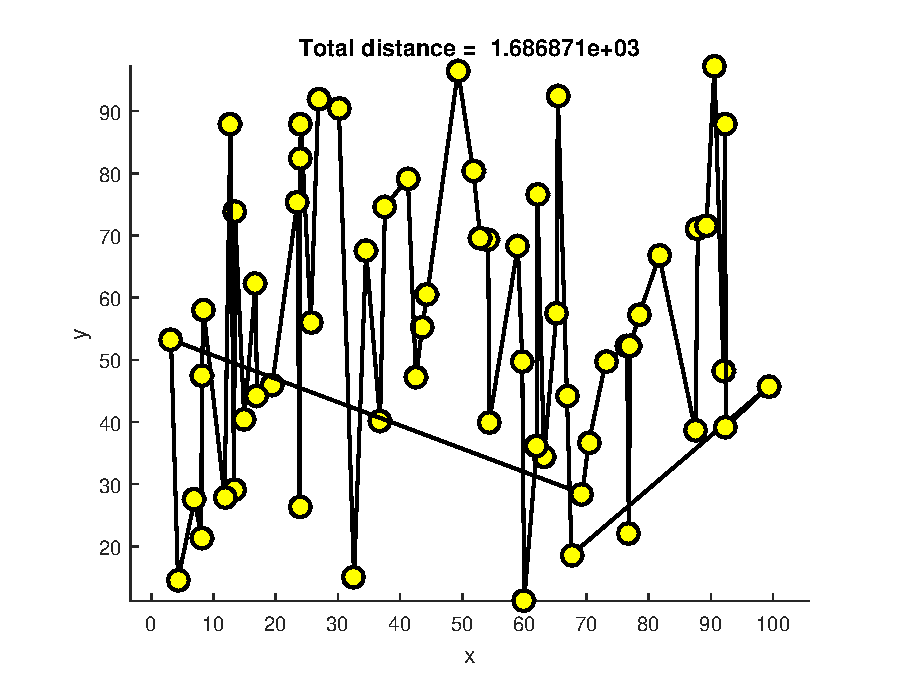
\includegraphics[width=\textwidth]{\Pathofsix/path.eps}
		\caption{Path journey}\label{fig:Pathofsix:path}
		
		\end{minipage}\hfill
		\begin{minipage}[t]{0.45\linewidth}
		\centering
		\includegraphics[width=\textwidth]{\Pathofsix/AS_1_5AS_ExecTimeAndMeanSTDWith_execVariation.eps}
		\caption{Variation of the execution time VS the \# of ants (20$\stackrel{step=20}{\rightarrow}$100) in each execution (1$\stackrel{step=1}{\rightarrow}$ 5)}
		\label{fig:Pathofsix:AS_1_5AS_ExecTimeAndMeanSTDWith_execVariation}
		\end{minipage}
		\flushleft
		\begin{minipage}[t]{0.45\linewidth}
		\centering
		\includegraphics[width=1.5\textwidth]{\Pathofsix/AS_BestCost_Varying_Iteration_and_nbAnts.eps}
		\caption{Best cost VS Ants number variation with $\alpha$=1, $ \beta $ = 5}
		\label{fig:Pathofsix:AS_BestCost_Varying_Iteration_and_nbAnts}
		\end{minipage}
\end{figure}
		\begin{minipage}[t]{0.9\linewidth}
		\vspace{-9mm}
		\begin{table}[H]
		\label{tab:Pathofsix:expdeux}
		\begin{tabular}{lllll}
		\cline{1-2}
		\multicolumn{1}{|l|}{Best Costs results for experience 2}                                                           &  \multicolumn{1}{l|}{Elapsed Time, Mean, STD}                                             &  &  &  \\ \cline{1-2}
		\multicolumn{1}{|l|}{\begin{tiny}\begin{tabular}{|l|c|c|c|c|c|c|c|c|c|c|}
\hline
&\textbf{It :1}&\textbf{It :2}&\textbf{It :3}&\textbf{It :4}&\textbf{It :5}&\textbf{It :6}&\textbf{It :7}&\textbf{It :8}&\textbf{It :9}&\textbf{It :10}\\\hline
\textbf{exec :1}&722.04&722.04&722.04&717.16&717.16&682.93&682.93&682.93&682.93&682.93\\\hline
\textbf{exec :2}&714.47&714.47&705.30&705.30&705.30&705.30&703.25&703.25&699.32&681.75\\\hline
\textbf{exec :3}&745.85&701.98&701.98&701.98&701.98&701.98&701.98&699.66&699.66&699.66\\\hline
\textbf{exec :4}&714.25&667.50&667.50&657.11&657.11&657.11&657.11&657.11&657.11&657.11\\\hline
\textbf{exec :5}&677.45&677.45&677.45&677.45&677.45&677.45&677.45&677.45&677.45&677.45\\\hline
\textbf{exec :6}&668.72&668.72&668.72&668.72&668.72&668.72&668.72&668.72&668.72&668.72\\\hline
\textbf{exec :7}&687.25&645.63&645.63&645.63&645.63&645.63&645.63&645.63&645.63&645.63\\\hline
\textbf{exec :8}&689.81&664.05&664.05&664.05&655.03&655.03&655.03&655.03&655.03&655.03\\\hline
\textbf{exec :9}&677.43&677.43&677.43&664.47&664.47&649.08&649.08&649.08&649.08&649.08\\\hline
\textbf{exec :10}&694.51&668.56&656.68&656.68&656.68&650.95&650.95&650.95&650.95&650.95\\\hline
\end{tabular}
\end{tiny}} & \multicolumn{1}{l|}{\begin{tiny}\begin{tabular}{|l|c|}
\hline
&\textbf{Elapsed time}\\\hline
\textbf{exec :1}&1.25\\\hline
\textbf{exec :2}&2.17\\\hline
\textbf{exec :3}&3.12\\\hline
\textbf{exec :4}&4.04\\\hline
\textbf{exec :5}&4.99\\\hline
\textbf{exec :6}&9.66\\\hline
\textbf{exec :7}&14.43\\\hline
\textbf{exec :8}&18.97\\\hline
\textbf{exec :9}&23.59\\\hline
\textbf{exec :10}&47.31\\\hline
\textbf{ Mean}&12.95\\\hline
\textbf{ STD}&14.28\\\hline
\end{tabular}
\end{tiny} } &  &  &  \\ \cline{1-2}
																						  &                                                                     &  &  &  \\
																						  &                                                                     &  &  & 
		\end{tabular}
		\caption{Results of experience 2 on rand60.dat}
		\end{table}
		\end{minipage}	
% %\end{figure}